\section{Histogram-based processing}

\subsection{Image CDF}

Below snippet shows my code for computing CDF's of (histograms of) images.
The \texttt{img\_hist} function also works with float images due to the use of
\texttt{img\_as\_ubyte} from \texttt{skimage}.

\begin{minted}[linenos=true]{python}
def img_hist(img):
    return np.bincount(img_as_ubyte(img).ravel(), minlength = 256)
def cdf_from_hist(hist):
    return hist.cumsum() / hist.sum()
def img_cdf(img):
    return cdf_from_hist(img_hist(img))
\end{minted}

Using this function, I compute the CDF as plotted in \cref{fig:3.1}. The CDF
has the steepest slope in roughly the range 75..110 and again in the range
120..145. These two ranges likely correspond to the dark gray colors in the
background and the lighter gray colors on the child's jacket, respectively.

The CDF is mostly flat in the ranges 0..75 and 170..255, since the image
contains neither very black nor very white pixels.

\begin{figure}[H]
    \centering
    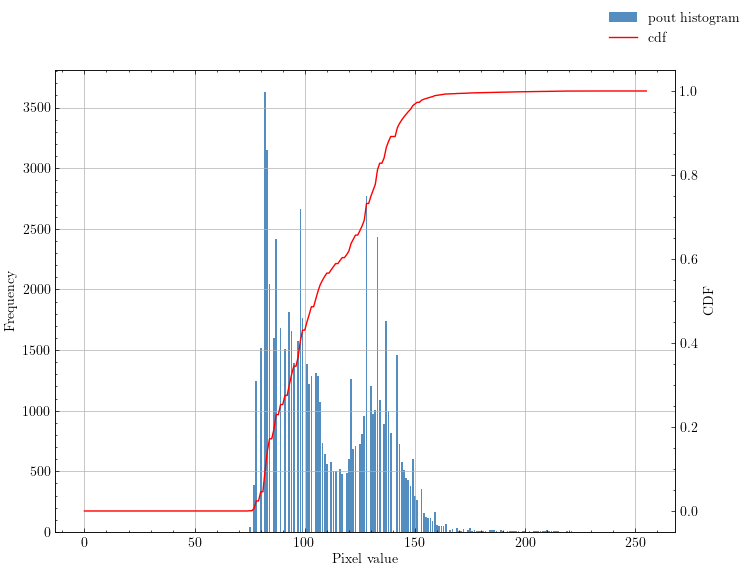
\includegraphics[width=0.7\textwidth]{figures/task_3_1.png}
    \caption{CDF (and histogram) of \texttt{pout.tif}.}
    \label{fig:3.1}
\end{figure}

\subsection{CDF substitution}

Below snippet shows my code for CDF substitution (as I call the process for lack
of a better term).

\begin{minted}[linenos=true]{python}
def cdf_substitution(img, cdf = None):
    return (cdf if cdf is not None else img_cdf(img))[img]
\end{minted}

The function takes an optional \texttt{cdf} argument; if not supplied, the
function computes the CDF from scratch. This CDF is then indexed using the
image, which is \emph{assumed to be an array of bytes}.

The result of applying the function to \texttt{pout.tif} is shown in
\cref{fig:3.2}.


\begin{figure}[H]
    \centering
    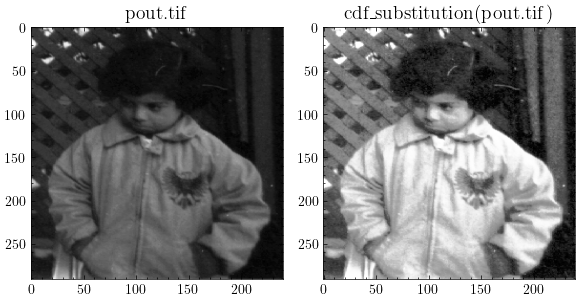
\includegraphics[width=0.7\textwidth]{figures/task_3_2.png}
    \caption{Result of applying CDF substitution to \texttt{pout.tif}.}
    \label{fig:3.2}
\end{figure}

\subsection{Pseudo-IDF}

The CDF is in general not invertible because it (in general) is not strictly
increasing, meaning multiple byte values may map to the same CDF values, and we
know that one criterium for invertibility is bijectivity. In fact, this is the
case for any image for which one or more values from the integer range $\{0,\
\dots,\ 255\}$ is \emph{not} represented in the byte representation of that
image.

Here is my Python code for computing the pseudo-IDF (pseudo-inverse distribution
function), or ``PIDF'', of an image given its CDF (or the image itself):
\begin{minted}[linenos=true]{python}
def pidf_from_cdf(cdf):
    return lambda ls: (cdf[:, None, None] >= ls).squeeze().argmax(0)
def img_pidf(img):
    return pidf_from_cdf(img_cdf(img))
\end{minted}

\texttt{pidf\_from\_cdf} works because \texttt{foo.argmax(0)} always returns the
index of the \textit{first} occurence of the argmax (as per the NumPy
documentation) along the 0'th axis. 


\subsection{Histogram matching}

My code for histogram matching:

\begin{minted}[linenos=true]{python}
# matches img_src to img_target's cdf.
def hist_match(img_src, img_target):
    return img_pidf(img_target)(cdf_substitution(img_src))
\end{minted}

The function replaces each pixel from \texttt{img\_src} by its CDF value using
the \texttt{cdf\_substitution} function from task 3.2, then feeds this result
into the pseudo-IDF of \texttt{img\_target} to create the histogram matching of
\texttt{img\_src} onto \texttt{img\_target}.

\Cref{fig:3.4.a} shows the result of histogram matching with
\texttt{pout.tif} and \texttt{trui.png} as source and target, respectively. To
verify my solution, I perform the same histogram matching using the \texttt{skimage}
implementation of histogram matching.

\begin{figure}[H]
    \centering
    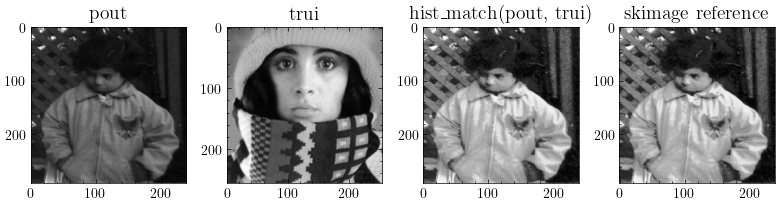
\includegraphics[width=\textwidth]{figures/task_3_4_matches.png}
    \caption{Result of matching \texttt{pout.tif} onto the histogram of
    \texttt{trui.png}, with \texttt{skimage.exposure.match\_histograms} for
    reference.}
    \label{fig:3.4.a}
\end{figure}


\Cref{fig:3.4.b} shows the histograms and CDF's for the source, target, and the
matching.

From these histograms we see that the range of significantly represented pixel
values in \texttt{pout.tif} is much smaller than that of \texttt{trui.png}, and,
equivalently, the CDF for \texttt{pout.tif} is much steeper in its increasing
range than the CDF for \texttt{trui.png}. This is evidenced by the actual
images: The spectrum of different colors in \texttt{pout.tif} is much smaller
than \texttt{trui.png}, and the colors are less dynamic and less contrasting.

Looking at the CDF and histogram of the matching, we see that the general shape
of the histogram and CDF resembles that of the \texttt{trui.png} histogram,
however here the histogram is significantly more sparse with big ``holes''
in-between the bars in the bar plot. A similar effect is seen in the CDF. This
is due to the significantly narrower dynamic range of \texttt{pout.tif}, as
mentioned above. As expected, the frequency values also resemble that of
\texttt{pout.tif}.

\begin{figure}[H]
    \centering
    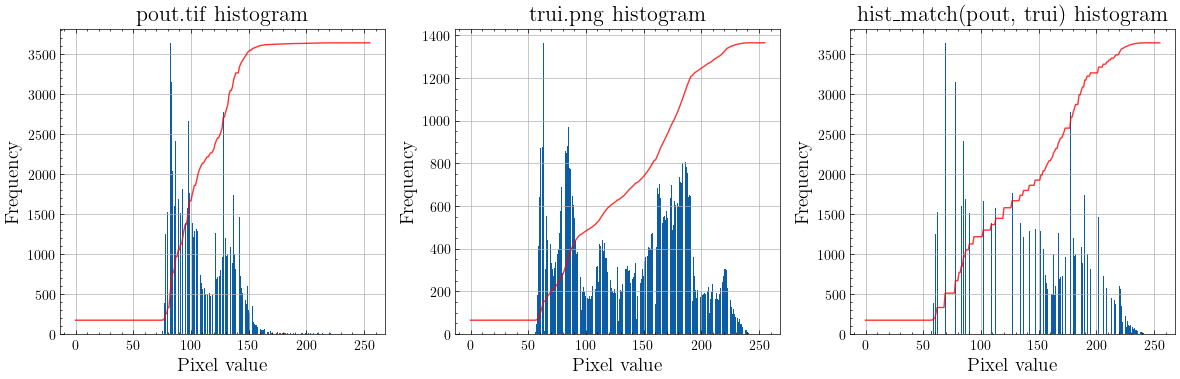
\includegraphics[width=\textwidth]{figures/task_3_4_histograms.png}
    \caption{Histograms and CDF's of \texttt{pout.tif}, \texttt{trui.png}, and
    the histogram matching of \texttt{pout.tif} onto \texttt{trui.png}.}
    \label{fig:3.4.b}
\end{figure}
